\begin{pastexam}[label={px:ncku-112-prog-03}]{成大資訊聯招 112 學年度 第 3 題}
（複選）

{[5\%]} Given a graph G as depicted as follows. T is minimum spanning tree (MST) of G. Which of the
following descriptions is (are) true?

\begin{center}
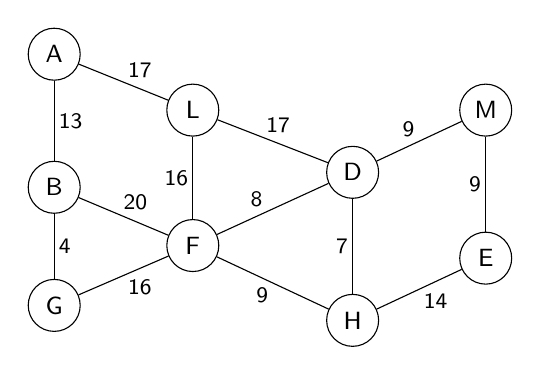
\begin{tikzpicture}[x=1cm,y=1cm,v/.style={circle,draw,inner sep=0pt,minimum size=6.6mm,font=\sffamily\small},w/.style={font=\sffamily\footnotesize,inner sep=1.5pt}]
\node[v] (A) at (0,0) {A};
\node[v] (L) at (1.76,-0.71) {L};
\node[v] (B) at (0,-1.69) {B};
\node[v] (D) at (3.79,-1.5) {D};
\node[v] (M) at (5.48,-0.71) {M};
\node[v] (F) at (1.76,-2.43) {F};
\node[v] (E) at (5.48,-2.59) {E};
\node[v] (G) at (0,-3.19) {G};
\node[v] (H) at (3.79,-3.38) {H};
\draw (A)--node[w,above right]{17}(L);
\draw (A)--node[w,right]{13}(B);
\draw (B)--node[w,right]{4}(G);
\draw (B)--node[w,above right,pos=0.45]{20}(F);
\draw (G)--node[w,below right,pos=0.5]{16}(F);
\draw (L)--node[w,left]{16}(F);
\draw (L)--node[w,above right,pos=0.4]{17}(D);
\draw (F)--node[w,above left,pos=0.45]{8}(D);
\draw (F)--node[w,below left,pos=0.5]{9}(H);
\draw (D)--node[w,left]{7}(H);
\draw (D)--node[w,above left,pos=0.5]{9}(M);
\draw (M)--node[w,left]{9}(E);
\draw (H)--node[w,below right,pos=0.5]{14}(E);
\end{tikzpicture}
\end{center}
\begin{enumerate}[label=(\Alph*)]
\item Perform Prim's algorithm to find the MST, starting from node L. The last edge included into the
MST is (A, B).
\item The minimum spanning tree for G is unique.
\item If let G2 be G by excluding the edge (M, E), then the G2's MST is identical to G's.
\item Let G3 be G2 removing the edge (B, F). The MSTs' of G2 and G3 are identical.
\end{enumerate}
\end{pastexam}

\begin{pastsoln}
答案：(A)(B)(D)。

圖有 $9$ 個頂點、$13$ 條邊：$AL$ 17、$AB$ 13、$BG$ 4、$BF$ 20、$GF$ 16、$LF$ 16、$LD$ 17、$FD$ 8、$FH$ 9、
$DH$ 7、$DM$ 9、$ME$ 9、$HE$ 14。

\textbf{(A) 對：Prim 從 L 開始}（資結書第~24.3~節）。 每一步加入跨過「樹內、樹外」的最輕邊：
\begin{center}
\small
\begin{tabular}{clll}
\toprule
步 & 樹內的點 & 跨過的候選邊（最輕的加粗） & 加入 \\
\midrule
1 & $L$ & $\mathbf{LF\,16}$，$LA$ 17，$LD$ 17 & $LF$ \\
2 & $L, F$ & $\mathbf{FD\,8}$，$FH$ 9，$GF$ 16，$LA$ 17，$LD$ 17，$BF$ 20 & $FD$ \\
3 & $+D$ & $\mathbf{DH\,7}$，$FH$ 9，$DM$ 9，$GF$ 16，$LA$ 17，$BF$ 20 & $DH$ \\
4 & $+H$ & $\mathbf{DM\,9}$，$HE$ 14，$GF$ 16，$LA$ 17，$BF$ 20 & $DM$ \\
5 & $+M$ & $\mathbf{ME\,9}$，$HE$ 14，$GF$ 16，$LA$ 17，$BF$ 20 & $ME$ \\
6 & $+E$ & $\mathbf{GF\,16}$，$LA$ 17，$BF$ 20 & $GF$ \\
7 & $+G$ & $\mathbf{BG\,4}$，$LA$ 17，$BF$ 20 & $BG$ \\
8 & $+B$ & $\mathbf{AB\,13}$，$LA$ 17 & $AB$ \\
\bottomrule
\end{tabular}
\end{center}
第 $3$ 步 $FH$ 9 和 $DM$ 9 一樣重，但 $DH$ 7 更輕，先加入；之後 $FH$ 的兩端都在樹內，不再是候選。 每一步
的最輕邊都唯一，所以順序是確定的，最後加入的是 $(A, B)$。 $T$ 的總重
$16 + 8 + 7 + 9 + 9 + 16 + 4 + 13 = 82$。

\textbf{(B) 對：唯一}。 資結書第~24.1.7~節：最小生成樹不唯一，若且唯若有一條不在 $T$ 裡的邊 $e$，它和
$T$ 上連接它兩端的路徑中某條邊一樣重（可以互換）。 逐一看不在 $T$ 的五條邊：
\begin{itemize}
\item $FH$ 9：$T$ 上 $F$ 到 $H$ 的路徑 $F$--$D$--$H$，最重 $8$，$9 > 8$。
\item $HE$ 14：路徑 $H$--$D$--$M$--$E$，最重 $9$。
\item $LD$ 17：路徑 $L$--$F$--$D$，最重 $16$。
\item $AL$ 17：路徑 $A$--$B$--$G$--$F$--$L$，最重 $16$。
\item $BF$ 20：路徑 $B$--$G$--$F$，最重 $16$。
\end{itemize}
每條都比路徑上的最重邊嚴格重，沒有可以互換的，所以 $T$ 唯一。

\textbf{(C) 錯}。 $ME$ 在 $T$ 裡，拿掉後 $E$ 只能靠 $HE$ 14 接回去（$E$ 只剩這條邊）。 $G2$ 的最小生成樹是
$T - \{ME\} + \{HE\}$，總重 $82 - 9 + 14 = 87$，和 $T$ 不同。

\textbf{(D) 對}。 $BF$ 20 本來就不在 $G2$ 的最小生成樹裡（它是環 $B$--$F$--$G$--$B$ 上最重的邊，環性質），
拿掉它不影響：$G3$ 的最小生成樹和 $G2$ 的一樣，都是 $T - \{ME\} + \{HE\}$。 （$G2$ 的最小生成樹也唯一，
同 (B) 的檢查方法。）
\end{pastsoln}
